% 文中引用说明

\chapter{相关技术理论}

\section{神经网络技术}

\subsection{循环神经网络}

\subsection{长短期记忆}

\section{GAN生成模型选取使用}
\subsection{基础GAN模型的缺陷}
GANs模型的缺点对应着优点,比较明显。由于GANs模型自由度太高,在面对过于清晰的图片等训练样本时,收敛性表现较差,生成模型可能出现退化,重复生成相同样本点,导致判别器无法工作,进而导致模型崩溃。因此,在训练过程中,调整好两个模型网络的平衡与同步非常重要。

正因为GAN模型有着这诸多的缺点,所以要选取比较合适的GAN模型来生成图片。

\begin{figure}[b]
    \centering
    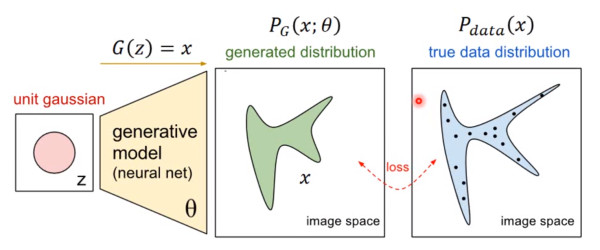
\includegraphics[width=0.8\textwidth]
    {figures/ganprograss.jpeg}\\
    \caption{一般GAN网络模型结构}
    \label{fig:GAN}
  \end{figure}

\subsection{衍生模型分类与特点}
目前对抗生成网络的衍生模型众多,其优化方式大抵由两个大方向衍生而来。一个方向是由损失函数的改变来优化GAN模型的效果,另一个方向则是从模型使用的角度来优化GAN模型的效果。在表~\ref{tab:1.1}中,列举了一些最为常见的GAN模型衍生模型。

\begin{table}[!htb]
    \centering
    \caption{}
    \label{tab:1.1}
    \begin{tabular}{cccc}
        \toprule
        从损失函数角度&\multicolumn{3}{c}{从模型应用角度提出的优化GAN模型}\\
        \cline{2-4}
        提出的优化GAN模型\upcite{fgans}&网络构架角度\upcite{mirza2014conditional}&编码器角度&其他角度改进\\
        \hline
        \multirow{5}{0.3\textwidth}{Least Square GANs, Loss-Sensitive GAN, Fisher GAN, WGAN, WGAN-GP, WGAN-LP, f-GANs\upcite, DRAGAN等}&\multirow{5}{0.19\textwidth}{CGAN, DCGAN, InfoGAN, StackGAN\upcite{zhang2017stackgan}, AL-GAN等}&\multirow{5}{0.19\textwidth}{BEGAN, VAE-GAN, tDCGAN, BiGAN,文献中的算法\upcite{编码器GAN1, 编码器GAN3, 编码器GAN2}等}&\multirow{5}{0.19\textwidth}{LAPGAN, ESRGAN, SRGAN, 3D-GAN, MGAN等}\\ \\ \\ \\ \\
        \bottomrule
    \end{tabular}
\end{table}

图像生成的模型与基于网络构架优化的GAN网络模型最为贴合,本文设计使用StackGAN作为基础,并针对相关实现进行优化。

\subsection{StackGAN及其衍生模型}
Han Zhang et al.在2017年提出了StackGAN模型,创新性地提出了基于栈的对抗式生成网络模型从文本生成图片的方法。

StackGAN和CGAN同属于优化了GAN网络的构架结构的一类GAN模型的分支。其中,StackGAN是对相对朴素的CGAN模型的优化。

\subsubsection{从CGAN到StackGAN}
条件对抗生成网络(Conditional GAN, CGAN)是Mirza\upcite{mirza2014conditional}于2014年提出的,如公式\eqref{eq:CGAN}表述,对生成模型和判别模型输入文本信息作为条件,使用了一个隐藏层的全联通网络(MLP)结构,实现了通过文字标签生成图像的功能。但是,CGAN的模型结构简单,效果差,收敛速度慢。在CGAN中,我们将文本作为条件输入生成器和判别器来训练两个模型生成和判别图像。如图~\ref{fig:cgan手写数字}和图~\ref{fig:萌娘}所示,及时CGAN应用广且有趣,但图像较小,质量不高。最基础的CGAN算法只能生成$64\times64$像素的图片,经过后来的改进,也只能将图片质量提升到$128\times128$像素。
\begin{equation}
  \min_G\max_DV(G,D)=\mathbb{E}_{x\sim P_{data(x)}}[\lg D(x_i\mid y)]+\mathbb{E}_{x\sim P_G(z)}\lg [(1−D(G(z_i\mid y)))]
  \label{eq:CGAN}
\end{equation}

\begin{figure}[!htb]
  \centering
  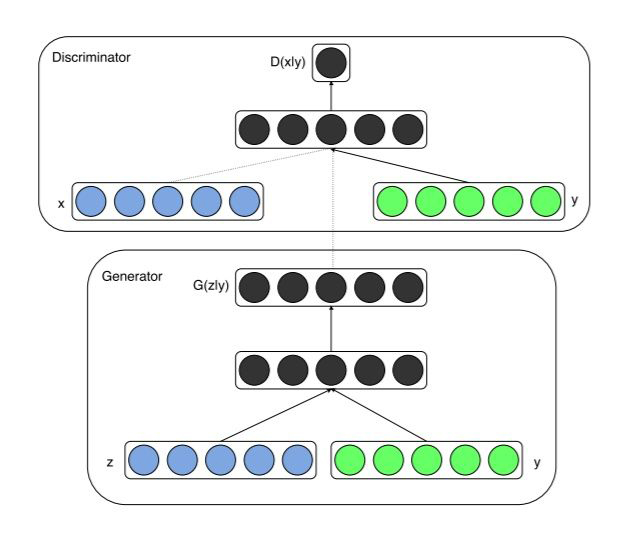
\includegraphics[width=0.5\textwidth]{figures/cgan.jpg}\\
  \caption{CGAN构架示意\upcite{mirza2014conditional}}
  \label{fig:CGAN}
\end{figure}

\begin{figure*}[htbp] 
  \centering 
  \begin{minipage}[c]{0.6\textwidth} 
    \begin{minipage}[c]{1\textwidth}
      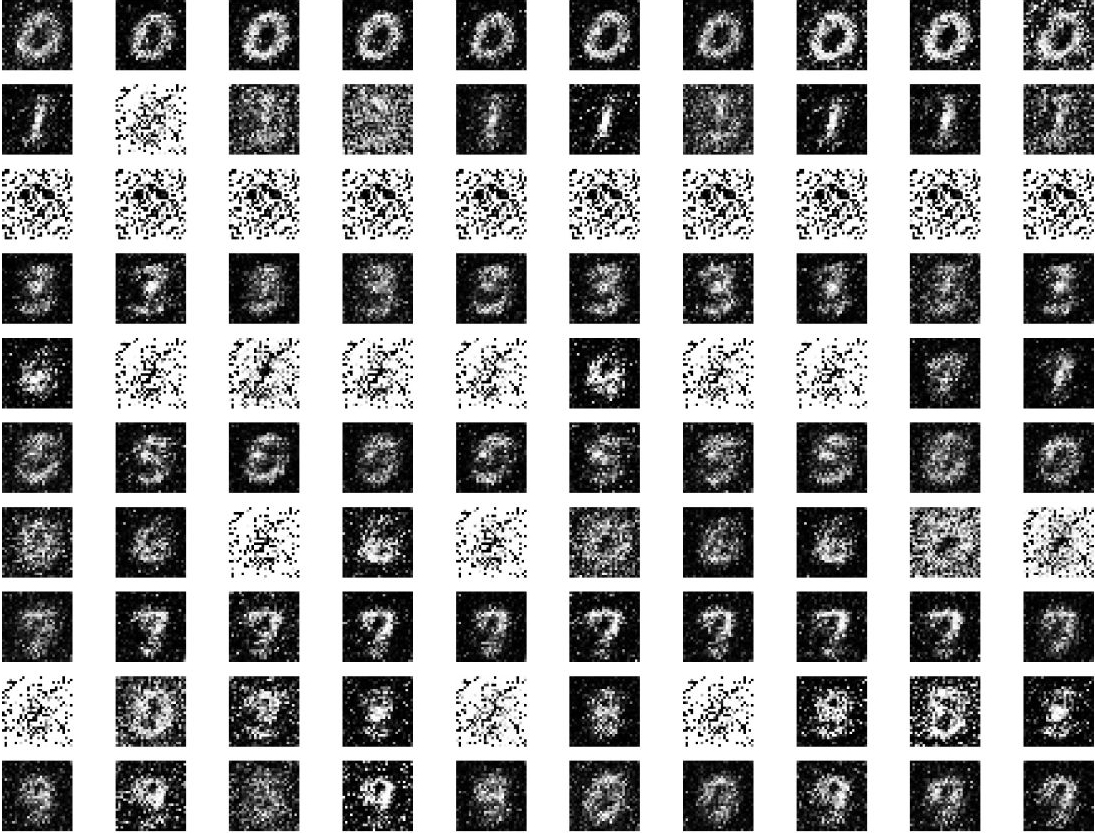
\includegraphics[width=0.45\textwidth]{figures/cgan手写数字1.jpg}\hspace{0.5em}
      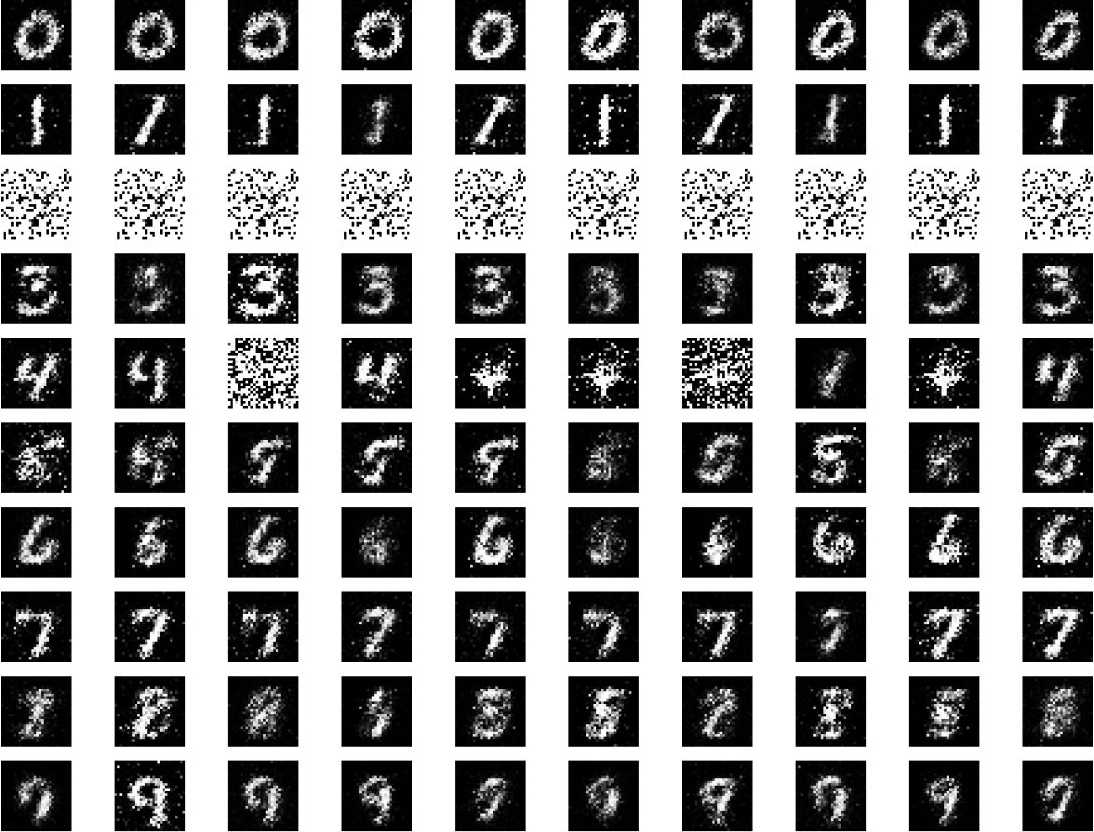
\includegraphics[width=0.45\textwidth]{figures/cgan手写数字2.jpg}
    \end{minipage} 
    \hfill \\ \vspace{-0.5em}\\
    \begin{minipage}[c]{1\textwidth}
      \hspace{0.2em}
      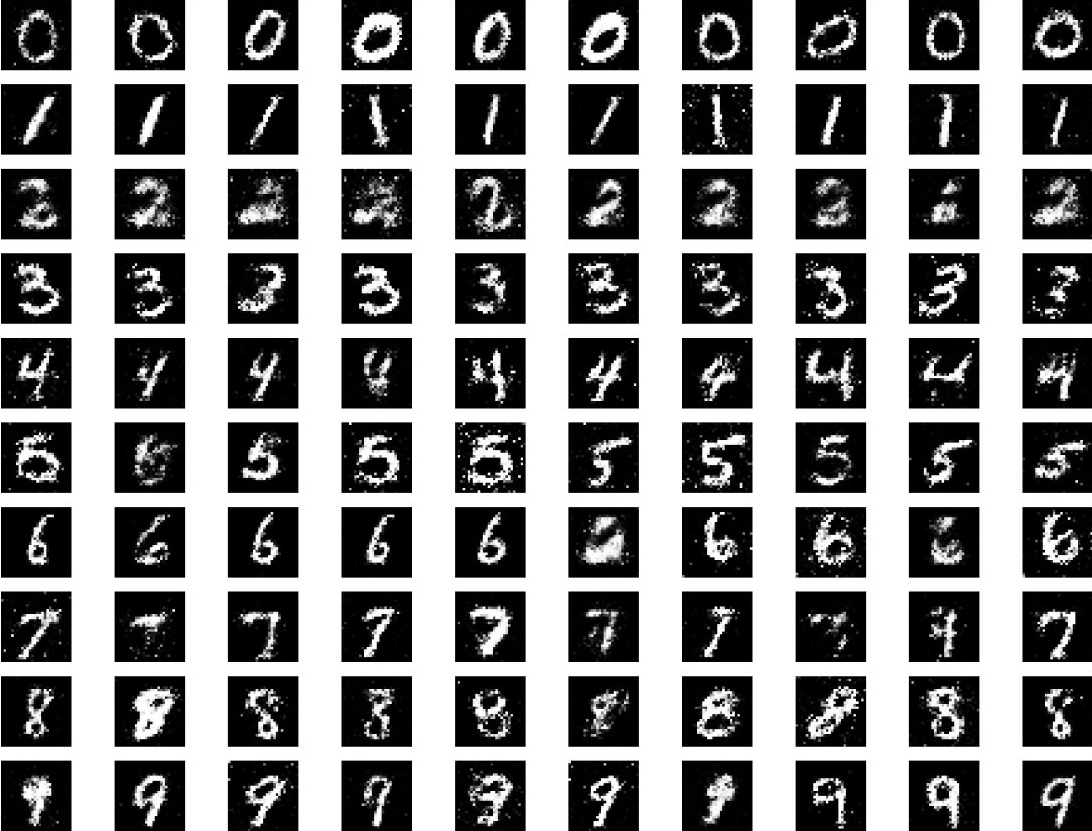
\includegraphics[width=0.45\textwidth]{figures/cgan手写数字3.jpg}\hspace{0.5em}
      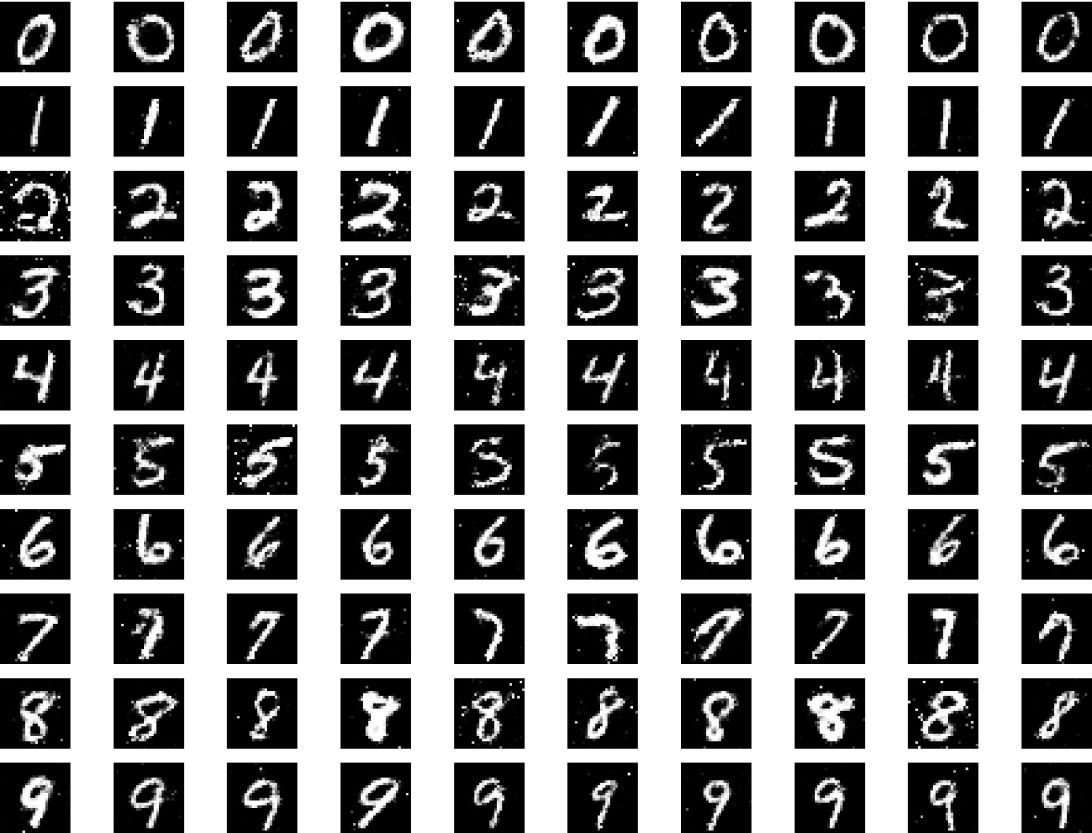
\includegraphics[width=0.45\textwidth]{figures/cgan手写数字.jpg}
    \end{minipage}
  \caption{CGAN生成手写数字\upcite{mirza2014conditional}(分别经历1、10、100、1000 个epoch后的结果)} %,zhihucgan
  \label{fig:cgan手写数字} 
  \end{minipage}
  \hfill 
  \begin{minipage}[c]{0.3\textwidth} 
  \centering%该小页居中排放图片 
  %\vspace{2em}
  \centerline{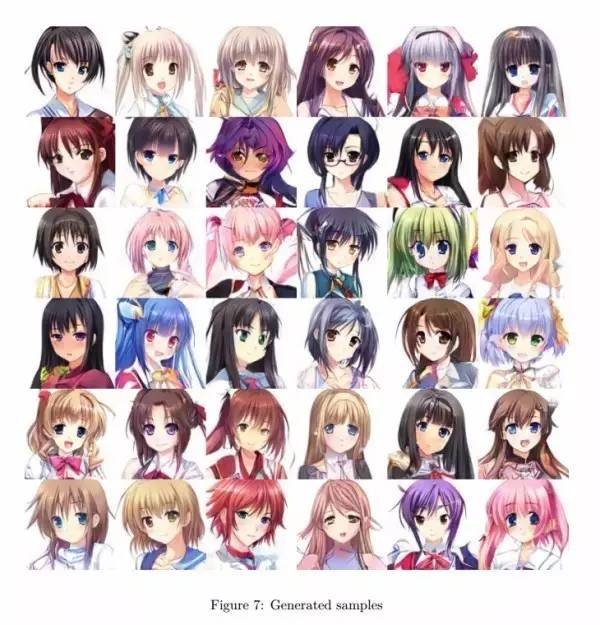
\includegraphics[width=1\textwidth]{figures/moegirl.jpg}}
  %\vspace{2em}
  \caption{CGAN生成二次元头像\upcite{2017comike}} 
  \label{fig:萌娘} 
  \end{minipage} 
  \end{figure*}

  为了解决这一问题,Han Zhan\upcite{zhang2017stackgan}在2016年提出了StackGAN模型,使用基于栈的结构,分两步进行训练。
  
  如图~\ref{fig:StackGAN}所示,第一步先训练模型使模型生成$64\times 64$像素的图片,训练出的模型只能输出像素低、形状有所扭曲的图片。第一次训练的时候并不使用转化为向量的文字直接作为输入,因为这一向量为1024维,过于稀疏,不利于深度的训练。在经历一次FC以后进行输入,这样可以增强表现。
  第一阶段训练的损失函数为式\eqref{stackgan_loss1}所示。
  第二次训练并不增加噪声输入,经过多轮残差网络迭代,
  %残差网络可以实现梯度的跨层传播,解决深度网络里面梯度消失的问题
  模型修正一轮训练生成图片的错误,并且在图像中添加细节,生成$256\times256$像素的“高清图片”。
  第二阶段训练的损失函数如式\eqref{stackgan_loss2}所示。
  \begin{equation}
    \begin{aligned}
      &&\mathcal{L}_{D_0} = & \mathbb{E}_{(I_0,t) \sim P_{data}}[\lg D_0 (I_0,\varphi_t)] \\ && &+\mathbb{E}_{z\sim P_z,t \sim P_{data}}[\lg (1-D_0(G_0(z, \hat{c}_0 ),\varphi_t))],
      \\
      &&\mathcal{L}_{G_0} = & \mathbb{E}_{z\sim P_z,t \sim P_{data}}[\lg (1-D_0(G_0(z, \hat{c}_0 ),\varphi_t))]  \\ && &+\lambda D_{KL}(\mathcal{N}(\mu_0(\varphi_t),\Sigma_0(\varphi_t))\parallel \mathcal{N}(0,I))
      \end{aligned}
    \label{stackgan_loss1}
  \end{equation}
  \begin{equation}
    \begin{aligned}
      &&\mathcal{L}_{D} = & \mathbb{E}_{(I,t) \sim P_{data}}[\lg D (I,\varphi_t)] \\ && &+\mathbb{E}_{s_0\sim P_{G_0},t \sim P_{data}}[\lg (1-D(G(s_0, \hat{c} ),\varphi_t))],
      \\
      &&\mathcal{L}_{G} = & \mathbb{E}_{s_0\sim P_{G_0},t \sim P_{data}}[\lg (1-D(G(s_0, \hat{c} ),\varphi_t))]  \\ && &+\lambda D_{KL}(\mathcal{N}(\mu(\varphi_t),\Sigma(\varphi_t))\parallel \mathcal{N}(0,I))
      \end{aligned}
    \label{stackgan_loss2}
  \end{equation}
    
  \begin{figure}[!htb]
    \centering
    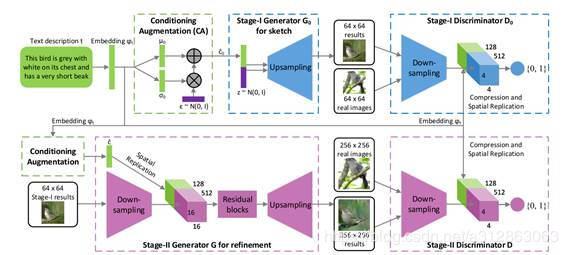
\includegraphics[width=0.9\textwidth]{figures/StackGAN.jpg}\\
    \caption{StackGAN构架示意}
    \label{fig:StackGAN}
  \end{figure}


  StackGAN模型相比较于CGAN模型,可以生成更高清的图片,而且

\subsubsection{对StackGAN的进一步优化与运用}
同一课题组紧接着提出了StackGAN++\upcite{zhang2018stackgan++},对原有算法进一步进行了优化。StackGAN++模型也叫做StackGAN\_v2,对之前的StackGAN模型主要有三点改进。第一,改为采取树状结构作为输入,通过不同的生成器来生成不同尺寸的图片,多层次叠加形成了有位置关系的“假图片”,即混合图层叠加图片;第二,额外引入了非条件性的损失,直接将服从正态分布的损失$z$叠加在最后生成的“假图片”上;第三,引入了色彩限制,限制了最终“假图片”的色彩信息分布。

李飞飞课题组的Johnson\upcite{Johnson_2018}在StackGAN模型之上,提出了自己的优化。

\section{本章小结}
本章中我主要总结了本次技术方案的前置技术,包括神经网络中的LSTM-RNN长短期记忆循环神经网络模型和StackGAN模型及其相关技术。LSTM-RNN模型是一种相对稳定、收敛,可以一定程度上避免梯度消失的深度学习模型,主要为下一章实现图片标注方法的技术做好铺垫。StackGAN及其升级版本是Han Zhang及其他科研人员2016年其后提出的一系列理论,我简要介绍了它的背景、原理和与后续技术的比较,决定使用李飞飞课题组的场景图像生成方法作为实现的理论依据,也为下一章自然语言生成图片的方法做好了前置说明。